\documentclass{standalone}
\usepackage{tikz}
\usepackage{amsmath}
\usetikzlibrary{math}
\usetikzlibrary{automata}

\newcommand{\mbf}[1]{\mathbf #1}
\newcommand{\mcal}[1]{\mathcal #1}
\newcommand{\eff}{\textrm{eff}}
\newcommand{\myOplus}[4]{
  \node[name=#1, circle, radius=1, draw,] at  (#2,#3) {};
  \draw (#1.north) -- (#1.south);
  \draw (#1.west) -- (#1.east);
  \draw[<-] (#1.north) -- ++(0,0.2) node[above] {$\mbf z_{#4}$};
}
\begin{document}
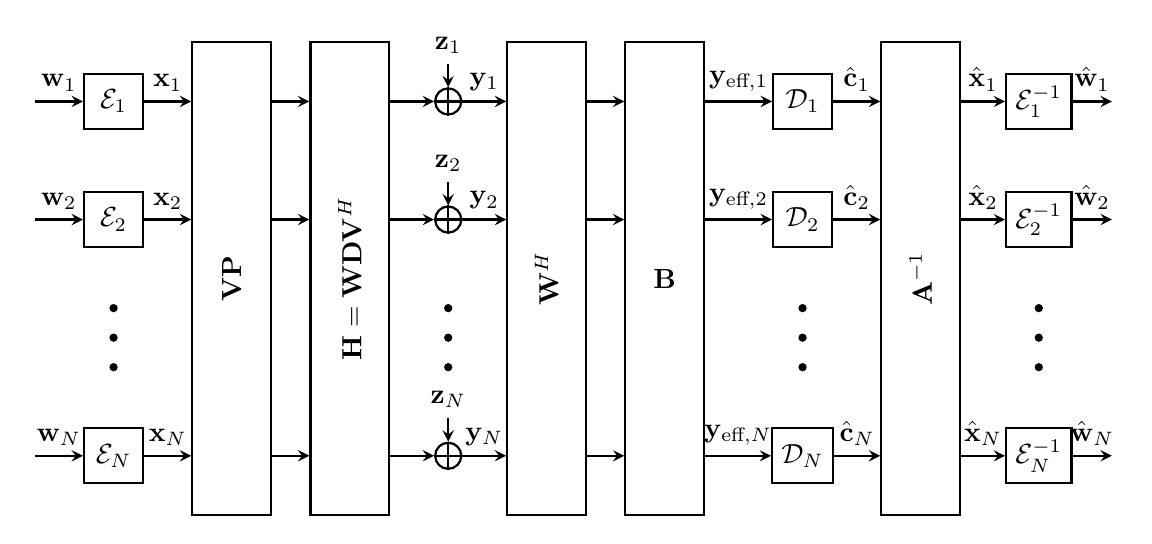
\begin{tikzpicture}[>=stealth, y=1.5cm, thick]
  \tikzset{smallbox/.style = { draw, rectangle, minimum width = 0.75cm, minimum height = 0.7cm }}
  \tikzset{bigbox/.style={ draw, rectangle, minimum height=1.5*4cm, minimum width=1cm}}
  \tikzset{textbox/.style={ rotate=90}}
%  \draw [gray, very thin] (0,0) grid (14,5);
%  \path [gray, very thin] (0,0) grid (14,5);
  % \foreach \x in {1,...,14} \node at (\x,0) {\x};
  % \foreach \y in {1,...,5} \node at (14,\y) {\y};
  
  \node[name = encN, smallbox] at (1,1) {$\mcal E_N$};
  \node[name = enc2, smallbox] at (1,3) {$\mcal E_2$};
  \node[name = enc1, smallbox] at (1,4) {$\mcal E_1$};

  \draw [->] (0,1) -- (encN) node[midway, above]{$\mbf w_N$};
  \draw [->] (0,3) -- (enc2) node[midway, above]{$\mbf w_2$};
  \draw [->] (0,4) -- (enc1) node[midway, above]{$\mbf w_1$};

  
  \fill (1,2) circle (1.5pt) +(0,0.25) circle(1.5pt) +(0,-0.25) circle(1.5pt);
  
  \node[name = P, bigbox] at (2.5,2.5){};
  \node[textbox] at (2.5,2.5){$\mbf{V} \mbf P$};

  
  \draw [->] (enc1) -- (enc1-|P.west) node[midway, above]{$\mbf x_1$};
  \draw [->] (enc2) -- (enc2-|P.west) node[midway, above]{$\mbf x_2$};
  \draw [->] (encN) -- (encN-|P.west) node[midway, above]{$\mbf x_N$};
  
  \node[name = H, bigbox] at (4,2.5){};
  \node[textbox] at (4,2.5){$\mbf H = \mbf W \mbf D \mbf V^H$};
  
  \draw [->] (enc1-|P.east) -- (enc1-|H.west);
  \draw [->] (enc2-|P.east) -- (enc2-|H.west);
  \draw [->] (encN-|P.east) -- (encN-|H.west);
  
  % \node[name=c1, circle, radius=1cm, draw] at  (0,0) {};
  % \draw (c1.north) -- (c1.south);
  \myOplus{z1}{5.25}{4}{1}
  \myOplus{z2}{5.25}{3}{2}
  \myOplus{zN}{5.25}{1}{N}

  \fill (5.25,2) circle (1.5pt) +(0,0.25) circle(1.5pt) +(0,-0.25) circle(1.5pt);
  
  \draw [->] (z1-|H.east) -- (z1);
  \draw [->] (z2-|H.east) -- (z2);
  \draw [->] (zN-|H.east) -- (zN);

  \node[name = W, bigbox] at (6.5,2.5){};
  \node[textbox] at (6.5,2.5){$\mbf{W}^H$};

  \draw [->] (z1) -- (z1-|W.west) node[midway, above]{$\mbf y_1$}; 
  \draw [->] (z2) -- (z2-|W.west) node[midway, above]{$\mbf y_2$};
  \draw [->] (zN) -- (zN-|W.west) node[midway, above]{$\mbf y_N$};

  \node[name = B, bigbox] at (8,2.5){$\mbf{B}$};

  \draw [->] (z1-|W.east) -- (z1-|B.west);
  \draw [->] (z2-|W.east) -- (z2-|B.west);
  \draw [->] (zN-|W.east) -- (zN-|B.west);

  \node[name = DecN, smallbox] at (9.75,1) {$\mcal D_N$};
  \node[name = Dec2, smallbox] at (9.75,3) {$\mcal D_2$};
  \node[name = Dec1, smallbox] at (9.75,4) {$\mcal D_1$};

  \draw [->] (B.east|-Dec1) -- (Dec1) node[midway, above]{$\mbf y_{\eff,1}$};
  \draw [->] (B.east|-Dec2) -- (Dec2) node[midway, above]{$\mbf y_{\eff,2}$};
  \draw [->] (B.east|-DecN) -- (DecN) node[midway, above]{$\mbf y_{\eff,N}$};
  
  \fill (9.75,2) circle (1.5pt) +(0,0.25) circle(1.5pt) +(0,-0.25) circle(1.5pt);

  \node[name = A, bigbox] at (11.25,2.5){};
  \node[textbox] at (11.25,2.5){$\mbf{A}^{-1}$};

  \draw [->] (Dec1) -- (Dec1 -| A.west) node[midway, above]{$\hat{\mbf c}_{1}$};
  \draw [->] (Dec2) -- (Dec2 -| A.west) node[midway, above]{$\hat{\mbf c}_{2}$};
  \draw [->] (DecN) -- (DecN -| A.west) node[midway, above]{$\hat{\mbf c}_{N}$};

  \node[name = inv1, smallbox] at (12.75,4) {$\mcal E_1^{-1}$};
  \node[name = inv2, smallbox] at (12.75,3) {$\mcal E_2^{-1}$};
  \node[name = invN, smallbox] at (12.75,1) {$\mcal E_N^{-1}$};
  
  \fill (12.75,2) circle (1.5pt) +(0,0.25) circle(1.5pt) +(0,-0.25) circle(1.5pt);

  \draw [->] (A.east |- inv1) -- (inv1) node[midway, above]{$\hat{\mbf x}_{1}$};
  \draw [->] (A.east |- inv2) -- (inv2) node[midway, above]{$\hat{\mbf x}_{2}$};
  \draw [->] (A.east |- invN) -- (invN) node[midway, above]{$\hat{\mbf x}_{N}$};

  \draw [->] (inv1.east) -- +(0.5,0) node[midway, above]{$\hat{\mbf w}_{1}$};
  \draw [->] (inv2.east) -- +(0.5,0) node[midway, above]{$\hat{\mbf w}_{2}$};
  \draw [->] (invN.east) -- +(0.5,0) node[midway, above]{$\hat{\mbf w}_{N}$};
\end{tikzpicture}
\end{document}
%%% Local Variables:
%%% mode: latex
%%% TeX-master: t
%%% End:
